%% ----------------ATENCIÓ-----------------------
%% Aquest document està preparat per codificació 
%% UTF-8. Si es llegeix amb un editor 
%% preparat per una altra codificació alguns 
%% caràcters no es veuran correctament.
%%---------------------------------------------- 
%%
%% Aquest document vos pot servir de base per la
%% realització de la memòria del treball final de
%% grau. Es recomana seguir els consells que 
%% apareixen en els diferents comentaris del 
%% document. Convindrà mantenir l'estructura
%% d'aquest exemple i introduir canvis sols 
%% allà on s'indiqui.
%%
%%-----------------------------------------------
%%
%% La plantilla preparada per a la realització de
%% la memòria és la classe LaTeX TFGEPSUIB.cls
%% que es fonamenta en la classe memoir. Aquesta
%% emula alguns `packages` que, per tant, no serà
%% necessari incloure dins el vostre document. El
%% manual de memoir explica quins són aquests
%% paquets (per exemple booktabs, array, tabluarx). 
%% Per altra banda, TFGEPSUIB també carrega 
%% automàticament els paquets, fontenc, xcolor, 
%% graphicx i microtype.
%%
%%-----------------------------------------
%% Opcions de la classe TFGEPSUIB:
%%
%% Per defecte, la classe TFGEPSUIB suposa
%% que la memòria es redactarà en català i que 
%% els estudis són els de Grau en Enginyeria
%% telemàtica. 
%%
%% Si preferiu utilitzar el castellà o anglés
%% per a la redacció de la memòria podeu
%% fer-ho indicant-ho a les opcions.
%\documentclass[catalan]{TFGEPSUIB}
\documentclass[spanish,GINF]{TFGEPSUIB}
%%
%% Per indicar quins són els estudis pels quals
%% es redacta la memòria heu d'incloure una de
%% les següents opcions:
%%
%% GTEL - Grau en Enginyeria Telemàtica
%% GMAT - Grau de Matemàtiques
%% GINF - Grau d'Enginyeria Informàtica
%% GEDI - Grau d'Enginyeria d'Edificació
%% GELE - Grau d'Eng. Elec. Ind. i Automàtica
%% GAGR - Grau en Eng. Agroali. i del Medi Rural
%%
%% Per escriure la memòria en castellà pels estudis
%% de matemàtiques, la línia inicial serà
%\documentclass[spanish,GMAT]{TFGEPSUIB}
%%------------------------------------------

% Indicau la codificació que usau en
% cas que no sigui UTF. 
%\usepackage[latin1]{inputenc}

% Per incloure expressions matemàtiques en
% el document és recomanable usar els paquets
%\usepackage{amsmath,amssymb,mathtools} 

% Per incloure fragments de codi hi ha diferents
% paquets disponibles. Triau el que vos sigui 
% més convenient, per exemple listings. 
%\usepackage{listings} 

% Amb tcolorbox podeu definir caixes per llistats,
% teoremes, exemples, ...
%\usepackage{tcolorbox}

% Si voleu que les referències bibliogràfiques
% apareguin amb el format "autor-any" en comptes 
% de "número" heu d'usar el paquet natbib.
%\usepackage[round,colon,sort&compress]{natbib} 

% En general, la documentació tècnica pot
% incloure molts acrònims. Per això es recomana
% usar el següent paquet. Consultau el corresponent
% manual per saber com s'usa.
\usepackage[printonlyused]{acronym}

% Les diferents unitats de mesura tenen un
% format estàndard de representació que convé
% respectar. Per això s'usa el paquet `siunitx`.
% També permet representar nombres en notació
% científica i alinear correctament els valors 
% numèrics a les taules. Pegau una ullada al 
% manual. Si no voleu usar-lo comentau la línia. 
\usepackage{siunitx}

% Com que és convenient que el paquet hyperref
% sigui un dels darrers en carregar-se, si voleu 
% afegir nous paquets, feis-ho a continuació.
%\usepackage{}

% El paquet "hyperref" crea enllaços automàticament 
% dins el document. Aquests enllaços permeten la 
% navegació a través de les diferents referències 
% figures, bibliografia, fórmules, índex, ...
% tant sols assenyalant-los amb el ratolí. 
\usepackage[draft=false, backref, hyperindex, plainpages=false, breaklinks=true, bookmarksnumbered=true]{hyperref}

% Aquests enllaços, per defecte, apareixen com a 
% requadres de diferents colors, el que resulta molt 
% pràctic en la versió electrònica del document.
% Aquests requadres NO apareixen en la 
% versió impresa. 

%----------------------------------------------
% Dades de la Portada amb els valors adequats
% La portada inclou informació del estudis,
% títol del projecte, autor(s) del projecte,
% tutor(s) (i supervisor(s)) i data. Títol,
% autor i tutor són dades obligatòries. El
% supervisor és opcional i la data també, però
% per defecte sempre apareix la del dia.
% Aquests valor s'han de definir si es vol usar
% la comanda \portada o \maketitle.
%
% Els estudis ja s'han definit amb la opció
% corresponent, però si el projecte
% és d'uns altres estudis no definits a les
% opcions, com són, per exemple, els dels plans
% anteriors, sempre podeu usar la comanda \estudis
% per definir-los.
% Per exemple, per l'enginyeria tècnica en 
% telemàtica podeu usar:
%\estudis{\MakeUppercase{Enginyeria Tècnica en Telecomunicacions, especialitat Telemàtica}}

\estudis{\MakeUppercase{Grado en Ingeniería informática}}

% Aquí podeu posar el títol de la vostra memòria
\title{Generador pseudo-aleatorio de trayectorias}

% Es recomana posar el nom de l'autor en 
% majúscules. Es pot fer automàticament amb la
% comanda \MakeUppercase. Si hi ha més d'un autor
% es poden separar mitjançant la comanda \and.
% Basta substituir els personatges de rondalla
% pels vostres noms.
\author{\MakeUppercase{Ahmed Antonio Boutaour Sanchez}}

% La comanda \tutor mostra el nom del director
% a la portada. Si hi ha més d'un tutor
% es poden separar mitjançant la comanda \and.
\tutor{Isaac Lera Castro}

% La comanda \supervisor permet incloure el nom 
% del professor de la UIB que avala el treball,
% en el cas que el director no sigui professor
% de la UIB.Si hi ha més d'un supervisor es poden 
% separar mitjançant la comanda \and. És una 
% comanda opcional
%\supervisor{Pere Catorze \and Joanet de Sa Gerra }

% Per defecte, la data apareix en el format 
% "dia de mes de any". Si vols que sols aparegui 
% el més pots activar i modificar la línia
%\date{juliol de 2012}

%---------------------------------------------------------------------------------------------------------------------------------------------------------------

% Durant l'escriptura de la memòria haureu de 
% compilar-la moltes vegades. Si voleu guanyar
% una mica de temps, podeu dividir el contingut
% en diferents fitxers i compilar-ne sols alguns.
% La comanda següent és la que vos permet
% definir quins compilar i quins no.
%\includeonly{Instruccions,Annexos}

% Quan vulgueu treballar amb tot el document, 
% simplement, comentau la línia anterior.  

%\addto\captionsspanish{\def\nomprojecte{Proyecto Fin de Carrera}}
\begin{document}


% Recordau haver indicat, títol, autor i tutor
% abans d'usar la comanda següent
\portada

% No toqueu la línia següent 
\frontmatter

% Si després de la portada voleu incloure una 
% pàgina de títol, podeu activar la línia
%\maketitle

% Voleu dedicar i agrair el treball a algú?
% Activau les línies següents i escriu el
% que vulguis dins l'entorn 'agraiments' 
%
%\cleartorecto \thispagestyle{empty}
%\begin{agraiments}
%%Posau aquí tot el que vulgueu
%\end{agraiments}

% A continuació el Sumari
\cleartorecto \tableofcontents

% Si voleu que apareguin una llista de figures
% i taules, activau les línies corresponents
%\cleartorecto \listoffigures
%\cleartorecto \listoftables 

% Si apareixen molts acrònims a la documentació
% convindrà fer-ne una llista. Podeu veure com
% crear-la consultant el fitxer 'Acronims.tex',
% que és el que s'inclou aquí.
\chapter{Acrònims} %Respectau títol del capítol.
%
% Per utilitzar els acrònims es recomana fer un poc 
% de recerca bibliogràfica per entendre com 
% funcionen. Concretament podeu llegir el manual
% que teniu dins el vostre sistema.
% La comanda `texdoc acronym` hauria de mostrar-lo.
%
\begin{acronym}

\acro{AMC}[AMC]{Adaptive Modulation and Coding}

\acro{EPS}[EPS]{Escola Politècnica Superior}

\acro{IP}[IP]{Internet Protocol}

\acro{LTE}[LTE]{Long Term Evolution}

\acro{MIMO}[MIMO]{Multiple-Input Multiple-Output}

\acro{OFDM}[OFDM]{Orthogonal Frequency Division Multiplexing}

\acro{OFDMA}[OFDMA]{Orthogonal Frequency Division Multiple Access}

\acro{RDI}[R+D+I]{Recerca, Desenvolupament i Innovació}

\acro{TCP}[TCP]{Transport Control Protocol}

\acro{TDMA}[TDMA]{Time Division Multiple Access}

\acro{TFG}[TFG]{Treball Final de Grau}


\end{acronym}
 
% Si no usau acrònims, comentau la línia anterior

% En l'arxiu Resum.tex es posarà el resum
% del treball.
%!TeX root=MemoriaTFG.tex

\chapter{Resum}

La capacitat de redacció i presentació oral de treballs científics i tecnològics és una de les competències més importants per al desenvolupament personal i professional d'un científic o d'un enginyer. Per tal de millorar aquestes competències, aquest document presenta una breu introducció a les habilitats que s'han de treballar per tal de ser un bon comunicador en qualsevol de les activitats acadèmiques i professionals.

Atès que en l'àmbit universitari la normativa del \ac{TFG} ens obliga a la redacció d'una proposta i d'una memòria de \ac{TFG} i a la defensa oral d'aquest treball davant d'un tribunal, en aquest document s'utilitza el \ac{TFG} com a exemple per introduir els principis bàsics per a la redacció i presentació de treballs. Tanmateix, les recomanacions que s'hi fan són prou generals com perquè puguin ser fàcilment esteses a altres activitats de comunicació científico-tecnològica.

D'una banda, a partir de la normativa de \acsp{TFG} de l'\ac{EPS} es descriuen les diferents etapes que s'han de superar fins a la defensa oral del \ac{TFG} i de l'altra, s'intenta donar resposta a preguntes del tipus: Què és el que fa que la documentació o la presentació oral d'un treball siguin bones? Quines són les millors passes a fer per redactar una bona documentació o per preparar una bona presentació? Quina ha de ser l'estructura global de la documentació o de la presentació?  

% No toqueu la línia següent 
\mainmatter\pagestyle{ruled}

%%%%%% COS DEL TREBALL %%%%%%%%%%%%

% Una bona pràctica consisteix en dividir
% un document llarg en diferents fragments,
% per exemple per capítols, i incloure aquests
% fragments dins el fitxer principal amb la
% comanda \include. Així, podem escriure la 
% comanda \includeonly{llista fitxers a compilar}
% que ens permetrà processar sols aquella part
% del document que ens interessi.

%!TeX root=MemoriaTFG.tex

\chapter{Introducció}

Els professionals de la comunicació tenen molt clar que \emph{la manera com s'explica una història és tan important com la pròpia historia}. No n'hi ha prou amb el fet de tenir una bona idea, un projecte de negoci extraordinari o uns resultats molt interessants, si no som capaços de presentar-los d'una manera adequada, el més probable és que no arribin a bon port.

\emph{Tant en l'àmbit acadèmic com en el laboral, saber comunicar d'una manera efectiva ens obrirà moltes portes}. En ambdós àmbits, tindrem idees, planejarem projectes o obtindrem resultats que, d'una manera o altra, haurem d'explicar als professors i companys d'una assignatura, als membres d'un tribunal acadèmic, als membres del gabinet tècnic d'una empresa, a un possible client o al nostre cap de secció. De l'\emph{impacte} que produeixi la nostra explicació (oral o escrita) en dependran, entre d'altres,
\begin{itemize}
 \item \emph{en l'àmbit acadèmic}: l'acceptació a tràmit i la valoració d'una tesi, l'obtenció de finançament per realitzar un projecte de recerca o la publicació d'un article en un congrés o en una revista i,
 \item \emph{en l'àmbit laboral}: l'aprovació del pressupost per a un projecte de part de la gerència de l'empresa, la signatura d'un contracte de serveis amb una altra empresa, la renovació del nostre contracte laboral, l'obtenció de subvencions per engegar un projecte de \acsu{RDI} o la nostra posició de lideratge.
\end{itemize}
Així doncs, atesa la seva rellevància per al nostre desenvolupament personal i professional, és important que ens esforcem per millorar les nostres capacitats de redacció i presentació de treballs científics i tecnològics.

El camp de la comunicació científico-tecnològica és molt ampli, amb tendències teòriques molt diverses, quantitats ingents de llibres i articles sobre el tema i, fins i tot, programes universitaris de grau i de postgrau. Per raons òbvies, doncs, aquest document no pretén abastar tot aquest camp, ni tan sols substituir la lectura d'altres referències bibliogràfiques molt recomanables. Només pretén fer una breu introducció a les habilitats que s'han de treballar per tal de ser un bon comunicador en qualsevol de les activitats acadèmiques i professionals pròpies d'un científic o d'un enginyer. La millora de les nostres habilitats de comunicació es traduirà en la millora dels nostres projectes i de les organitzacions en què treballem i, potser més important, en la millora de la nostra satisfacció personal i de les nostres carreres acadèmiques i professionals.

En l'àmbit universitari el \acf{TFG} constitueix una part important dels estudis de grau. L'objectiu fonamental d'aquest treball, tot i que sovint requereix estudis addicionals en un camp determinat, és que els estudiants apliquin els coneixements, les habilitats i les competències adquirides en els seus estudis de grau a la resolució d'un problema aplicat. Atesa l'obligatorietat de la presentació d'una proposta i d'una memòria de \acf{TFG} i de la defensa oral d'aquest treball davant un tribunal acadèmic, centrarem els continguts d'aquest manual en la introducció dels principis bàsics per a la redacció i presentació d'aquest tipus de treballs. Tanmateix, intentarem que les recomanacions siguin prou generals com perquè puguin ser fàcilment esteses a altres activitats de comunicació científico-tecnològica.

Dedicarem el capítol \ref{instruccions} a fer una petita descripció de les instruccions generals i l'itinerari a seguir per a la realització del \ac{TFG}. Als capítols \ref{proposta} i \ref{memoria} ens centrarem, respectivament, en els aspectes formals de la redacció de la proposta i de la memòria del \ac{TFG}. En el capítol \ref{presentació} descriurem els principis bàsics i les bones pràctiques per a la realització de la defensa oral del \ac{TFG} davant del tribunal. Acabarem amb una secció que recollirà les conclusions més importants d'aquest manual.


%!TeX root=MemoriaTFG.tex

\chapter{Instruccions generals i itinerari del Treball Final de Grau }\label{instruccions}
\begin{figure}
\centering
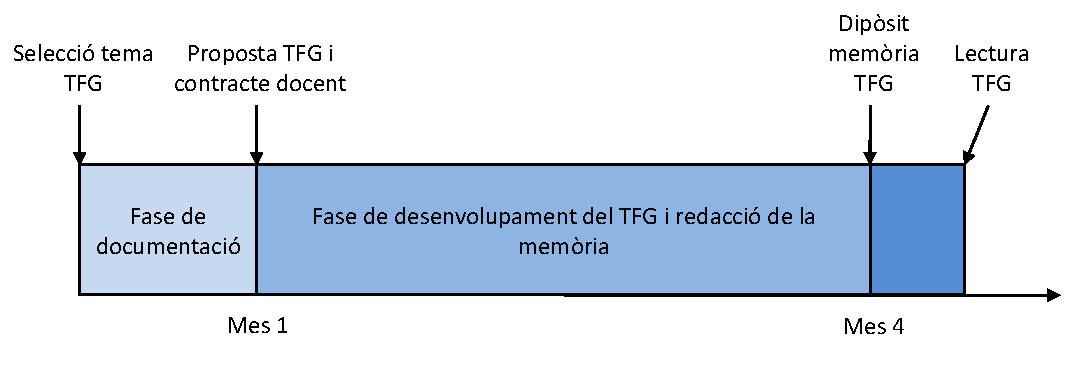
\includegraphics[width=\linewidth]{./Imagenes/Itinerari_TFG.pdf}
\caption{\label{fig:itinerari}Itinerari del Treball Final de Grau}
\end{figure}

\section{Inici del Treball Final de Grau}

Com a norma general, tal com apareix reflectit en els plans d'estudis de gairebé totes les titulacions de grau, el \ac{TFG} s'hauria de realitzar en el segon semestre de quart curs. Tanmateix, tot i que aquestes s'agrupen en cursos i semestres, els estudis universitaris s'estructuren en assignatures. Així doncs, atesa la naturalesa integradora del \ac{TFG}, la recomanació general seria que abans de començar a realitzar el \ac{TFG} haguéssim aprovat la major part de les assignatures troncals i obligatòries del grau. De fet, l'ideal seria que només ens manquessin les assignatures que en el pla d'estudis corresponent es cursen simultàniament amb el \ac{TFG}.

\section{Selecció del tema de Treball Final de Grau}

Una de les vies més habituals per escollir el tema de \ac{TFG} és a través de l'apartat corresponent de la web de l'\acf{EPS}. En aquest cas, després de revisar les propostes realitzades pels diferents professors o grups de recerca involucrats en la docència de l'\ac{EPS}, escollirem les que més ens interessin i contactarem amb els professors responsables. Si algun dels professors encara no té el tema assignat i ens accepta, començarem a treballar en la fase de documentació i en la preparació de la proposta.

Existeixen altres possibilitats a l'hora d'escollir un tema de \ac{TFG}. Per exemple, podem realitzar el \ac{TFG} en una empresa del sector. En aquest cas és important que contactem amb un professor de l'\ac{EPS} que vulgui realitzar les tasques de supervisió i que pertanyi a un àrea de coneixement propera als continguts a tractar en el \ac{TFG}, d'aquesta manera ens assegurarem que la proposta de \ac{TFG} i el camp que aquesta cobreix compleixen amb els estàndards habituals a la nostra titulació. En cas de dubte, el més convenient és contactar amb el cap d'estudis de la titulació corresponent que segur que ens orientarà i ens proporcionarà la informació necessària.

Val a dir que el \ac{TFG} també es pot realitzar en una universitat amb la que s'hagin establert convenis de convalidació (programes Sèneca, Erasmus, Averroes, \ldots). Tanmateix, en aquest cas haurem de seguir els procediments administratius establerts en aquesta altra universitat.

\section{Preparació de la proposta i contracte docent}

Un cop escollit el tema de \ac{TFG} començarem a treballar en la fase de documentació i, d'acord amb el nostre supervisor, prepararem la proposta de \ac{TFG}. Per a la redacció d'aquesta proposta convé seguir les indicacions descrites al capítol \ref{proposta} i és recomanable que aquesta fase de documentació i preparació de la proposta de \ac{TFG}, tal com es mostra a la Fig. \ref{fig:itinerari}, no s'allargui més enllà d'un mes. Sobre la proposta de \ac{TFG} és sobre la que estudiant i professor signaran el contracte docent. En aquest contracte s'establiran els compromisos del professor quant a seguiment i supervisió del projecte i els de l'estudiant quant a dedicació i termini de presentació. La proposta de \ac{TFG} i el contracte docent, signat tant per l'alumne com pel professor, seran lliurats als serveis administratius on l'\ac{EPS} signarà el compromís de disponibilitat de medis materials genèrics i de formalització d'un tribunal de \ac{TFG} adient.

\section{Desenvolupament del Treball Final de Grau}

Un cop aprovada la proposta de \ac{TFG} ens dedicarem a la realització del \ac{TFG} i a la redacció de la memòria sota la supervisió del director i seguint les condicions estipulades en el contracte docent. Per a la redacció de la memòria convé seguir les indicacions descrites al capítol \ref{memoria}. És recomanable que aquesta fase de desenvolupament i redacció del treball, tal com ens mostra la Fig. \ref{fig:itinerari}, no superi els quatre mesos.

\section{Dipòsit de la memòria}

Una vegada acabada la seva redacció, i amb el vist-i-plau del nostre supervisor, dipositarem la memòria del \ac{TFG} a secretaria seguint les indicacions de la normativa de \acsp{TFG} de l'\ac{EPS}.

\section{Preparació de la presentació}

Finalment només ens quedarà preparar la presentació del \ac{TFG} per tal de fer-ne la defensa oral davant el tribunal. Per a la preparació d'aquesta presentació convé seguir les indicacions del capítol \ref{presentació}.

% !TEX root=ManualTFG.tex

\chapter{La proposta de treball de final de grau}\label{proposta}

\section{Principis bàsics}
En un treball de final de grau ben planificat, la proposta de \ac{TFG} constituirà el primer document formal relatiu al projecte. A més, especialment amb la introducció del contracte docent relatiu al \ac{TFG}, la proposta assoleix una importància cabdal ja que aquest és el document sobre el qual estudiant, director i \ac{EPS} adquireixen compromisos respecte de la duració màxima del treball, tasques de supervisió, disponibilitat de materials, \ldots

La redacció d'una proposta ben definida i consensuada entre director i alumne suposa avantatges importants com, per exemple:
\begin{itemize}
\item Garanties de que, abans d'iniciar el desenvolupament del \ac{TFG}, l'alumne comprèn perfectament el problema que es vol abordar i és capaç de contextualitzar-lo, entenent com la temàtica del seu \ac{TFG} lliga amb la resta de coneixements de l'àrea.

\item Disponibilitat d'una descripció precisa dels objectius del \ac{TFG} i d'una estimació dels resultats que se n'esperen.

\item Visualització del full de ruta del \ac{TFG} que ha de permetre, tant al director com a l'alumne, l'avaluació del progrés en l'execució del projecte i en l'assoliment dels objectius.
\end{itemize}

En la major part dels casos, la proposta formal d'un \ac{TFG} es redactarà a partir d'una proposta de tema provinent d'un professor o d'un grup de recerca. Aquesta proposta de tema descriurà breument el context del treball, el problema adreçat i els objectius que s'intenten assolir. A més, hauria de proporcionar les referències i eines bàsiques a utilitzar i explicitar, també, els coneixements previs i habilitats recomanades per poder dur a terme el \ac{TFG}. El més desitjable seria que totes les propostes de temes de \ac{TFG} es fessin públiques a través de la web de l'\ac{EPS}, tanmateix és probable que també n'apareguin als taulers d'anuncis, portes dels laboratoris de recerca o les portes dels despatxos dels professors. És responsabilitat dels alumnes estar atents a la publicació d'aquests anuncis.

Es pot donar el cas d'alumnes que prefereixin realitzar el \ac{TFG} en una empresa o alumnes que estiguin especialment interessats en un àrea de coneixement concreta i ells mateixos vulguin proposar un tema de \ac{TFG}. En qualsevol d'aquests casos és important que trobin un supervisor i que discuteixin amb ell la preparació de la proposta formal de \ac{TFG}. En el cas de \ac{TFG}s desenvolupats en empreses serà important també comptar amb el vist-i-plau del director/tutor dintre de l'empresa.

El més habitual serà que l'alumne interessat en una proposta de tema de \ac{TFG} comenci llegint les referències bàsiques subministrades per tal d'assolir uns coneixements bàsics sobre el context general del tema proposat i poder plantejar el problema que es vol abordar i els objectius concrets que es persegueixen. Això, comptant amb el suport del supervisor del \ac{TFG}, ha de permetre passar a l'etapa de redacció de la proposta formal del \ac{TFG}. L'elaboració de la proposta pot implicar l'estudi de conceptes que no s'han cobert en els estudis de grau, la cerca de referències bibliogràfiques addicionals a les subministrades a la proposta del professor o l'avaluació d'eines \emph{hardware} i/o \emph{software} que no s'havien utilitzat abans.

La transició des de la proposta de tema del professor cap a la proposta formal de \ac{TFG} per part de l'alumne pot servir, també, per adaptar l'enunciat general d'un problema a un enunciat més específic que reculli les inquietuds de l'estudiant. A més, la proposta d'un professor o d'un grup de recerca pot acabar derivant en més d'una proposta de \ac{TFG} si hi ha més d'un alumne interessat en el tema i és possible estructurar-la en diversos \ac{TFG}s.

Finalment, és important recordar que la proposta de \ac{TFG} s'adjuntarà a un contracte docent entre director, alumne i \ac{EPS} i, per tant, ha d'estar consensuada entre les tres parts.


\section{La proposta de tema}

El format de la proposta de tema del professor serà bastant variable ja que dependrà molt del tipus de projecte concret a desenvolupar i també de l'\emph{estil} de cada professor. En qualsevol cas hauria de contenir informació suficient per a que l'alumne pugui tenir una idea prou clara de en què consisteix el projecte i quins objectius es persegueixen, de quins coneixements li faran falta per afrontar-ho i de quines són les referències bàsiques del tema, que poden servir com a punt de partida per entendre altres referències necessàries per redactar la proposta de \ac{TFG}.

Així, doncs, alguns elements importants que haurien de quedar reflectits a la proposta de tema són:
\begin{itemize}
\item Contextualització: La proposta de tema hauria d'incloure una breu introducció al context del \ac{TFG}, però suficientment detallada per facilitar què l'alumne pugui relacionar la feina a fer amb els coneixements adquirits al llarg dels estudis grau.
\item Definició d'objectius: S'haurien d'explicitar els objectius que es perseguiran en el projecte. El grau de concreció dels objectius dependrà del projecte en si: a vegades la proposta de tema ja suggerirà els resultats concrets que es pretén obtenir i en altres ocasions serà feina de l'alumne definir els objectius concrets del seu \ac{TFG}.
\item Bibliografia: A l'hora de proporcionar una llista de referències bibliogràfiques bàsiques s'ha de tenir en compta el nivell de coneixements dels alumnes potencialment interessats
    en el tema de \ac{TFG}. És molt probable que aquesta bibliografia bàsica estigui principalment composta de capítols de llibres i articles introductoris publicats en revistes i congressos.
\item Pre-requisits: La proposta de tema de \ac{TFG} també hauria d'especificar si el \ac{TFG} té pre-requisits en forma d'assignatures que és necessari haver cursat (o estar cursant), habilitats (e.g. programació de baix nivell, càlcul matemàtic) o interessos particulars dels alumnes.
\end{itemize}

La transició des de proposta de tema publicada per un professor o per un grup de recerca cap a la proposta de \ac{TFG} que ha de redactar l'estudiant, amb el suport del seu supervisor, és previsible que impliqui les passes següents:
\begin{itemize}
\item Immersió en el tema: L'alumne haurà de ser capaç de relacionar el tema del \ac{TFG} amb les assignatures que ha cursat durant els seus estudis de grau. Aquest procés ha d'ajudar a l'alumne a prendre consciència de quins coneixements bàsics li faran falta per dur a terme el \ac{TFG}. La bibliografia bàsica proporcionada a la proposta de tema ha de servir per a que l'alumne adquireixi els coneixements fonamentals per contextualitzar el seu treball.
\item Definició d'objectiu: Un cop assimilats els continguts de les referències introductòries s'ha de ser capaç de definir de manera ben concreta els objectius del \ac{TFG}. Per això pot ser necessària la consulta d'altres referències més especialitzades i/o la discussió d'alguns aspectes del treball amb el supervisor. Aquesta definició d'objectius també ha de servir, si és el cas, per incorporar a la proposta els interessos personals del projectista.
\item Programació temporal: Tenir objectius ben delimitats i ser conscients dels coneixements necessaris per dur-los a terme ha de permetre a l'alumne fer una programació temporal realista del \ac{TFG}. Serà important comprovar que aquesta programació temporal s'ajusta a la càrrega de feina que s'havia previst a la proposta de tema i a la càrrega en crèdits ECTS del \ac{TFG}. Si aquest no és el cas, serà necessari tornar a avaluar els objectius del projecte per determinar si aquests s'han d'ampliar o reduir. A l'hora de fer aquesta programació temporal és fonamental que el projectista tingui en compte la càrrega de feina addicional al \ac{TFG} (assignatures, pràctiques en empresa, \ldots). Els diagrames de PERT o GANT són eines útils per realitzar aquesta programació temporal.
\end{itemize}
Com ja s'ha mencionat abans, la proposta de tema pot donar lloc a més d'una proposta de \ac{TFG} si, per exemple, hi ha més d'un alumne interessat en el tema proposat. En aquest cas serà
responsabilitat del supervisor verificar que les diferents propostes, encara que parteixin d'un \emph{background} comú, tenen objectius concrets ben diferenciats.

\section{Estructura de la proposta de Treball Final de Grau}
En general l'estructura de la proposta de \ac{TFG} inclourà:
\begin{itemize}
\item \emph{Títol}: El títol ha de descriure de la manera més precisa possible el treball a realitzar. Aquest títol no ha de coincidir necessàriament amb el títol definitiu que apareixerà a la memòria.
\item \emph{Paraules clau}: La llista de paraules clau ha d'incloure els conceptes fonamentals que formen la base del \ac{TFG}. En cas de que eventualment s'arribi a disposar d'una base de dades de \ac{TFG}s, aquesta llista serà molt útil a l'hora de fer-hi cerques en funció dels temes tractats.
\item \emph{Context}: Aquesta secció ha de servir per situar el \ac{TFG} dins una determinada àrea de coneixement, per fer una descripció concisa sobre l'estat de l'art del tema sobre el que tractarà el \ac{TFG} i per aclarir els motius que han portat a la realització d'aquest treball. Hauria de servir, també, per introduir el plantejament general del problema que es pretén abordar. Els conceptes clau del projecte han d'aparèixer en aquesta secció definits de manera clara per tal de resoldre possibles ambigüitats i malentesos entre alumne i supervisor. És previsible que aquesta secció, juntament amb la dedicada als objectius, constitueixin la base del primer capítol de la memòria del \ac{TFG}.
\item \emph{Objectius}: En els objectius s'han de concretar les fites del treball tot indicant les qüestions específiques adreçades en el \ac{TFG} i els mètodes que s'empraran per donar-hi resposta. És important que siguin objectius mesurables, és a dir, que el seu assoliment sigui constatable.
\item \emph{Programació temporal}: La programació temporal descriurà el ritme i ordre en que s'han d'anar realitzant les diferents activitats. El nivell de detall de la planificació dependrà del que acordin alumne i supervisor quant a la periodicitat de les reunions des supervisió.
\item \emph{Eines}: Aquí s'explicitaran aquelles eines \emph{hardware} i/o \emph{software} que es faran servir per dur a terme el \ac{TFG}.
\item \emph{Bibliografia}. La bibliografia inclourà totes les referències bibliogràfiques rellevants en la redacció de la proposta de \ac{TFG}, tant les proporcionades en la proposta de tema com aquelles que s'hagin pogut descobrir durant els processos de documentació i redacció dels antecedents i objectius de la proposta final.
\end{itemize}

% !TEX root=MemoriaTFG.tex

\chapter{La memòria del treball de final de grau}\label{memoria}

\section{Principis bàsics}

\emph{Què és el que fa que una memòria de \ac{TFG} sigui bona?} Òbviament, la resposta a aquesta pregunta pot ser molt complexa, però hi ha molts autors (vegeu, per exemple, \cite{Perelman01,Malvar08} i els treballs que aquests referencien) que coincideixen en que un informe tècnic o científic ha de reunir les qualitats següents:
\begin{itemize}
   \item \emph{precisió}: aquesta qualitat es fonamenta en tres aspectes complementaris:
   \begin{enumerate}

   \item \emph{precisió del document}, que fa referència a que aquest s'ha de concentrar de forma precisa en el tema que el defineix i n'ha de fer un tractament correcte, basat en evidències científicament demostrables, i amb un nivell de detall apropiat, ni massa general ni excessivament restringit.

   \item \emph{precisió estilística}, que només és possible si es fa un ús curós del llenguatge per tal d'expressar el significat. La precisió en l'ús del llenguatge es fonamenta en el rigor en la utilització de les paraules, en una estructura correcta de les frases i en un ús adequat dels signes de puntuació.

   \item \emph{precisió tècnica}, que es fonamenta en un bon coneixement tècnic de la matèria i del seu vocabulari.
   \end{enumerate}

   \item \emph{concisió}: molt relacionada amb la precisió del document, la concisió es fonamenta en la focalització, és a dir, en la reducció de l'abast del document a l'àmbit estricte de la qüestió que es vol tractar. És molt fàcil caure en la temptació d'incloure en la memòria materials que potser són molt rellevants en el camp en què es desenvolupa el treball, però que no ho són en absolut per comunicar de manera efectiva les aportacions concretes del treball en aquest camp.
       %Com veurem més endavant, la definició precisa i detallada de l'índex de la memòria és una de les estratègies més útils per controlar la longitud i l'abast del document. També és important identificar i eliminar els materials (frases, paràgrafs, seccions, \ldots) que no són necessaris per recolzar o evidenciar les nostres aportacions. Les figures i les taules solen contribuir a la concisió del document perquè redueixen la quantitat de prosa necessària per descriure objectes i processos, resumeixen dades i serveixen per demostrar relacions.
%
   \item \emph{claredat}: aquesta qualitat, que fa referència a la capacitat de qui escriu per facilitar la comprensió del document a qui llegeix, és especialment important en l'escriptura científico-tècnica. Els vocabularis especialitzats, els desenvolupaments matemàtics o els esquemes conceptuals complexos poden dificultar moltíssim la comprensió d'algunes explicacions tècniques, fins i tot quan aquestes han estat redactades per escriptors especialitzats i són processades per lectors experts.

   \item \emph{coherència (organització i estructura)}: un document és coherent si el material que presenta està organitzat de manera lògica i consistent i la seva estructura proporciona al lector un camí fàcil per a la seva comprensió. La coherència es valora de forma molt especial en ciència i tecnologia degut a la inherent complexitat dels temes que es tracten.


   \item \emph{adequació a l'audiència}: és convenient que el document s'adeqüi als objectius que l'autor s'ha marcat a l'hora d'escriure'l, però, sobretot, és molt important que s'adeqüi a les necessitats dels possibles lectors (supervisors, membres del tribunal, altres alumnes que treballin en temes semblants, \ldots) i al context, objectius i convencions (forma i estil) de la institució en què es presenta.
\end{itemize}

Tal com ens recorda H. S. Malvar a \cite{Malvar08}, l'error més freqüent que podem cometre a l'hora d'escriure, especialment en el cas de l'escriptura científica, és no saber posar-nos al lloc del lector. Així doncs, la recomanació fonamental per evitar errors a l'hora d'escriure la memòria és que cada cop que afegim una nova argumentació, una nova figura o una nova taula, pensem en els possibles lectors d'aquesta informació i la revisem per tal de garantir que és precisa, clara, concisa, coherent i adequada a l'audiència.

\section{Bones pràctiques}

\emph{Quines són les millors passes a fer per escriure una bona memòria de \ac{TFG}?} La major part dels treballs de final de grau es desenvolupen en tres etapes, una primera etapa en què es duu a terme una revisió de les referències bibliogràfiques més rellevants sobre el context general i l'àmbit particular del projecte, una segona etapa en què es realitzen estudis analítics, simulacions, implementacions reals, \ldots i, finalment, una tercera etapa en què es redacta la memòria. Tanmateix, aquestes tres etapes no són estrictament consecutives i, habitualment, treuen profit d'una retroalimentació sistemàtica entre elles. En aquesta secció, tot i ser molt conscients d'aquesta interdependència, ens centrarem en l'etapa de redacció de la memòria i presentarem una sèrie de recomanacions a seguir en els processos de \emph{focalització}, \emph{elaboració de l'esbós} i \emph{redacció}.

\subsection{Focalització} Aquest procés aborda de ple les qualitats de precisió del document, concisió i adequació a l'audiència. La focalització consisteix en la reducció de l'abast del document a l'àmbit estricte que el defineix, en la selecció acurada dels temes sobre els que ha de tractar i en l'adequació dels continguts i profunditat de tractament d'aquests a l'audiència concreta a la que es vulgui dirigir. Per focalitzar un document, algunes de les passes que ens podrien servir serien:
\begin{enumerate}
   \item Fer una llista completa dels temes o paraules clau que defineixen el nostre treball.

   \item Si encara no ho hem fet, recórrer a les referències bibliogràfiques que calgui per tal de tenir una visió prou acurada del paper que juga cadascun d'aquests temes en el context general i en l'àmbit particular del tema que ens ocupa.

   \item A partir de la llista de temes i de la informació disponible sobre cadascun d'aquests, respondre a preguntes del tipus:
   \begin{itemize}
          \item És necessari que tracti aquest tema en la memòria?
          \item Es perdran els lectors de la memòria si no tracto aquest aspecte?
          \item Puc deixar de parlar sobre aquest tema sense perjudicar l'objectiu global del meu projecte?
          \item És excessivament general aquest tema o és excessivament específic?
          \item N'hi ha prou amb un tractament general acompanyat de referències bibliogràfiques o seria millor que el lector disposés d'una visió més detallada per tal de poder seguir els raonaments posteriors?
          \item És necessari introduir coneixements previs per poder tractar alguns dels temes de la llista?
   \end{itemize}
   Aquest tipus de preguntes actuaran com a filtres que ens permetran eliminar temes innecessaris, afegir-ne de necessaris o preveure la profunditat amb la que s'ha de tractar cadascun dels temes seleccionats. En haver acabat disposarem d'una bona eina per passar a l'etapa d'elaboració del primer esbós de la memòria.
\end{enumerate}

\subsection{Elaboració de l'esbós} Un cop hem focalitzat l'àmbit estricte del treball i, per tant, disposem de la llista de temes seleccionats i tenim una idea general de la profunditat amb què els volem tractar, una bona manera de facilitar el procés de redacció consisteix en la preparació d'un esbós detallat del nostre treball. Es comença amb una taula de continguts que conté un llistat dels títols provisionals dels capítols, seccions i subseccions que es volen incloure en la primera versió de la memòria. Després, per cadascun dels capítols, seccions i subseccions es redacten una sèrie de frases curtes que descriuen, de forma ordenada, els aspectes clau de tots i cadascun dels continguts que s'hi tractaran i, si es creu convenient, les fonts en les que ens podem recolzar en el procés de redacció. En aquestes etapes continua sent especialment important tenir en ment les qualitats de precisió, concisió i adequació a l'audiència de la nostra proposta, però també hi jugarà un paper especialment rellevant la qualitat de coherència. Paga la pena dedicar temps i esforç en l'elaboració d'aquest primer esbós i revisar-lo tantes vegades com sigui necessari fins a estar-ne totalment convençuts.

Un cop tenim l'esbós provisional del document és el moment de fer-ne una revisió acurada amb l'ajut del nostre supervisor. Aquesta revisió ens hauria de permetre, entre d'altres coses, eliminar el material innecessari, afegir el material o argumentacions que se'ns hagin pogut oblidar i reestructurar els continguts per tal d'incrementar el nivell de coherència del document. És més eficient i menys dolorós prendre aquestes decisions en les fases inicials del procés de redacció, que haver-les de prendre un cop ja s'ha escrit molt de material que al final s'ha de descartar. A partir d'aquest primer esbós ens resultarà més senzill visualitzar l'estructura global de la memòria i saber, en cada moment, quin és l'estat del procés de redacció. Ens permetrà determinar si el treball realitzat (simulacions, implementacions, anàlisis, \ldots), els resultats obtinguts i les referències bibliogràfiques consultades són suficients o si és necessari aprofundir en algun aspecte concret. Ens ajudarà, també, a planificar la nostra feina en funció del temps disponible.

\subsection{Redacció} L'estratègia de redacció a seguir a partir d'aquest primer esbós no ha de ser necessàriament lineal, és a dir, no ha de començar necessàriament amb la redacció del capítol d'introducció i acabar amb la del capítol de conclusions. De fet, tot i que és molt important partir d'una idea molt clara dels continguts del capítol d'introducció, atès que aquest és el que proporciona una visió global del context i l'abast del treball, en la majoria dels casos ens pot resultar més senzill començar amb la redacció dels capítols corresponents al desenvolupament del treball i acabar amb la redacció de la introducció i les conclusions. És l'anomenada estratègia \emph{de dintre cap a fora}.

És molt possible que, a mesura que anem redactant aquesta primera versió de la memòria, també descobrim que és necessari fer addicions, supressions i altres esmenes sobre l'esbós original a fi d'assolir-ne la versió definitiva. En qualsevol cas, atès que les frases curtes que hem utilitzat apunten, de forma ordenada i coherent, els aspectes clau de tots i cadascun dels continguts dels capítols, seccions i subseccions de la memòria, si ens dediquem a desenvolupar-les en forma de paràgrafs, recorrent, sempre que sigui necessari, a l'ajut de figures, taules, desenvolupaments matemàtiques, \ldots, al final obtindrem la primera versió de les diferents parts de la memòria.

La primera versió d'una secció o d'un capítol és la primera passa cap a la versió definitiva, però no ens ha de fer mandra revisar-la i reescriure-la tants cops com sigui necessari per tal de millorar-ne les qualitats de precisió, claredat, concisió, coherència i adequació. Aquest procés de revisió s'ha de fer a consciència, intentant descobrir paraules, frases, taules, figures o, fins i tot, paràgrafs que no contribueixen a que el text sigui més precís o més concís o més clar, procurant, també, millorar l'organització i l'estructura dels diferents elements que conformen el text i, no menys important, mirant d'aconseguir la precisió estilística a través de la correcció ortogràfica i gramatical.

La paraula clau és revisió i, com no podia ser d'altra manera, un cop donem per acabada la primera versió d'un capítol és el moment de que el nostre supervisor també la revisi. Atès que ja havíem mantingut reunions amb el supervisor per discutir l'esbós de la memòria, és poc probable que aquesta revisió suposi canvis substancials en l'estructura general del capítol. Tanmateix, hi pot haver aspectes del treball que només s'hagin tractat de manera més o manco informal i, per tant, la lectura d'aquesta versió pot ser el primer contacte formal del supervisor amb alguns dels plantejaments teòrics o pràctics realitzats per l'alumne. Així doncs, hi ha la possibilitat de que es detectin mancances o errors que suposin el replantejament d'alguns apartats. És molt important que considerem tots els suggeriments que ens faci el supervisor i que els utilitzem per millorar la següent versió de la memòria. Si s'han produït replantejaments d'algunes parts del treball pot ser necessària una segona revisió per part del supervisor.

Quan el supervisor hagi revisat tots els capítols de la memòria i nosaltres hàgim realitzat tots els canvis oportuns, només restarà portar a terme una revisió global de la memòria per tal d'obtenir-ne la versió definitiva.

\section{Estructura del Treball Final de Grau}

Tal com ens recorda el professor Valiente \cite{Valiente96}, organismes internacionals d'estandardització com l'ANSI (\emph{American National Standards Institute}) o la ISO (\emph{International Organization for Standardization}) prescriuen sistemes estàndard per a l'organització dels treballs científics que contenen quatre parts fonamentals: introducció, desenvolupament, resultats i conclusions. Aquestes parts fonamentals d'un treball científic es complementen amb altres components com la portada, la taula de continguts, les llistes de figures, taules i acrònims, el resum, els agraïments, els apèndixs o les referències bibliogràfiques.


\subsection{Portada}

La portada actua com a element de presentació i identificació del \ac{TFG}. Les dades que s'hi han de fer constar poden variar en funció del tipus de treball, però n'hi ha algunes que són fonamentals: títol, autors, directors i, si s'escau, tutors, departament, universitat, títol acadèmic al qual s'opta i data de presentació. Després de la portada s'acostumen a deixar un o més fulls en blanc de cortesia.

El títol és sens dubte una part molt important de la memòria del \ac{TFG}. És el primer lligam que s'estableix entre el \ac{TFG} i el lector i, per tant, s'ha de ser molt curós a l'hora de seleccionar les paraules i les frases que donaran forma al títol. Un bon títol és aquell que descriu el contingut del \ac{TFG} de manera precisa i amb el menor nombre de paraules possible. Una bona estratègia a l'hora d'escriure el títol del \ac{TFG} és partir d'una llista de paraules clau i tractar de trobar quines d'aquestes són fonamentals a l'hora de descriure la nostra aportació i quin ha de ser l'ordre i l'associació entre aquestes paraules clau. Òbviament, a mesura que anem escrivint la memòria podem anar manejant una sèrie d'alternatives que puguin donar lloc a diferents títols i deixar que amb el temps alguna d'elles es vagi imposant sobre les altres.

\subsection{Taula de continguts o Sumari}

La taula de continguts o sumari és un llistat dels títols dels diferents capítols, seccions i subseccions del document amb indicació dels números de pàgina en què apareixen. Per tant, la taula de continguts no només ajuda als lectors a cercar els diferents temes tractats en la memòria, sinó que també serveix com a esbós de l'estructura de la memòria i ofereix una visió general del document als lectors potencials. Òbviament, les taules de continguts més útils es componen de títols de caire descriptiu.

\subsection{Llista de figures}

Els lectors utilitzen la llista de figures per localitzar la informació visual en la memòria. La llista de figures relaciona els títols o llegendes dels recursos visuals (figures, dibuixos, fotografies, \ldots) amb la seva ubicació dintre de la memòria. És important que les llegendes de les figures siguin descriptives i que estiguin numerades de manera consecutiva.

\subsection{Llista de taules}

La llista de taules proporciona les llegendes i la localització de totes les taules que apareixen a la memòria. De la mateixa manera que els títols de figura, els títols o llegendes de les taules s'han de numerar consecutivament en l'ordre en què apareixen al document.

\subsection{Llista d'acrònims}

Hi ha documents que utilitzen una quantitat important de termes nous, o molts acrònims i abreviacions. En aquests casos es pot facilitar la lectura de la memòria si s'inclou una llista de nomenclatura o una llista d'acrònims just després de les llistes de figures i/o taules. Un dels efectes secundaris interessants de les llistes de nomenclatura o d'acrònims és que ajuden a l'autor del document a utilitzar la terminologia d'una manera coherent.

\subsection{Resum}

El resum és una breu declaració, generalment entre 250 i 500 paraules, que proporciona al lector una sinopsi del problema, el mètode, els resultats i les conclusions de la memòria. Els resums s'han de poder llegir de manera totalment independent de les altres parts de la memòria i, per tant, no s'hi han d'utilitzar acrònims sense definir-los i tampoc s'hi han d'utilitzar referències bibliogràfiques. Els resums són extremadament útils per aquelles persones que volen tenir una imatge general del contingut de la memòria abans de llegir el document principal. Atès que hi pot haver lectors potencials que utilitzin el resum per decidir si han de continuar llegint la memòria o no, cal no menystenir la importància d'una bona redacció d'aquest apartat del document. Els resums poden estalviar una immensa quantitat de temps als possibles lectors.

El resum ha d'incloure, com a mínim, els següents elements:
\begin{itemize}\tightlist
   \item Definició abreujada del problema o tema principal del \ac{TFG}.

   \item Exposició del mètode utilitzat per resoldre el problema.

   \item Comentaris sobre els principals resultats, aportacions i possibles aplicacions del treball.

   \item Conclusions més importants del treball
\end{itemize}

\subsection{Agraïments}

A vegades s'inclou una secció d'agraïments en els preliminars de la memòria per tal de donar crèdit a l'assistència rebuda de part de persones i/o institucions. Els supervisors, els tècnics de laboratori o els companys de feina que ens han assessorat o ens han donat suport són, tots ells, candidats a aparèixer al capítol d'agraïments.

\subsection{Introducció}

Si hem decidit utilitzar l'estratègia \emph{de dintre cap a fora}, després de redactar els capítols corresponents al desenvolupament del treball estarem en disposició d'enllestir la redacció de la introducció i les conclusions.

La introducció hauria de servir per donar, de forma descriptiva i fàcil d'entendre, una visió global del context i l'abast del treball. De fet, segons Booth~\emph{et al.}~\cite{Booth08}, el patró comú que cerquen els lectors en qualsevol introducció està format per tres elements:
\begin{itemize}
   \item Contextualització: es tracta d'explicitar el context en el que s'emmarca el treball, d'establir la base comuna de coneixements sobre el tema que es tractarà en la memòria del \ac{TFG}, de garantir que els possibles lectors comparteixen amb l'autor de la memòria el conjunt de factors que els permetran interpretar adequadament els seus enunciats i raonaments.

       El context d'un \ac{TFG} podria ser, per exemple, el món de les xarxes de comunicacions mòbils de quarta generació (4G), amb capes físiques basades en l'ús de múltiples antenes en transmissió i en recepció (\acsu{MIMO} -- \emph{\acl{MIMO}}), tècniques de codificació i modulació adaptatives (\acsu{AMC} -- \emph{\acl{AMC}}) i estratègies d'accés múltiple basades en l'ús de transmissió multiportadora (\acsu{OFDMA} -- \emph{\acl{OFDMA}}). En aquest cas seria adequat parlar sobre l'estat actual del desenvolupament dels estàndards 4G, de les característiques generals de les tecnologies \ac{MIMO}, \ac{AMC} i \acsu{OFDM}/\ac{OFDMA} i de la seva adequació als sistemes 4G. Depenent de l'àmbit d'aplicació del problema a tractar podria ser adequat aprofundir, per exemple, en la descripció de l'estat actual de les xarxes de comunicacions ce\lgem{}lulars i de les característiques de les estacions base i/o de les estacions repetidores o en la descripció de l'estat actual de les xarxes d'àrea local sense fils i de les possibles estratègies de cooperació entre punts d'accés.

   \item Definició del problema: un cop establert el context del treball, és l'hora de definir amb precisió el problema que es tractarà en el \ac{TFG} i de justificar la seva importància dintre del context en el que s'emmarca. Es tracta, també, de proporcionar una visió general, però concisa, dels antecedents del problema, de les publicacions més rellevants sobre el tema, de les virtuts i mancances dels plantejaments i solucions aportades per altres autors.

       Dintre del context de l'exemple anterior, un possible problema a resoldre en un \ac{TFG} podria ser, atesa la necessitat de gestionar els recursos disponibles d'una manera eficient, el de l'assignació òptima de potència, subportadores i modes de transmissió (codificació de canal i modulació) per tal de garantir una taxa de transmissió global màxima amb restriccions sobre la qualitat de servei proporcionada a les aplicacions dels diferents usuaris del sistema.

   \item Resposta al problema: després de definir el problema, el més lògic és presentar al lector de la memòria la nostra proposta per solucionar-lo, els nostres objectius. Es tracta d'explicitar el mètode seleccionat per solucionar el problema plantejat anteriorment, tot justificant aquesta selecció. També pot ser adequat avançar, tot i que de manera concisa, els resultats principals del \ac{TFG} i les possibles conclusions que es desprenen dels resultats obtinguts.

       En el problema de l'exemple anterior, una possible resposta podria consistir en el desenvolupament d'algorismes d'optimització dual, en l'ús de la teoria de jocs o, per posar-ne un altre exemple, en l'ús d'aprenentatge estadístic (\emph{machine learning}). En cadascun d'aquests casos hauríem de justificar la tria feta i, si ens semblés adient, podríem parlar de quins són els resultats que mostrarem al lector en el desenvolupament de la memòria del \ac{TFG}.

\end{itemize}


Avui en dia, tant en la universitat com en l'empresa, és molt habitual que el \ac{TFG} formi part de projectes de recerca més amplis, de manera que pot ser difícil per al lector discernir quan és que l'autor descriu el seu treball personal i quan és que descriu una tasca realitzada per altres membres del grup de recerca. En aquests casos, és molt important que l'autor expliciti el millor possible quin ha estat exactament el seu paper dintre d'aquest projecte general.

Tot i que hi ha autors que no ho recomanen, una manera habitual d'acabar una introducció consisteix en presentar un resum de l'estructura de la memòria, avançant al lector quins són els continguts dels diferents capítols del \ac{TFG}.


\subsection{Desenvolupament}

Aquesta part de la memòria, que es pot estructurar en diversos capítols, tracta sobre la pròpia realització del treball i descriu el que s'ha fet, com s'ha fet, per què s'ha fet d'aquesta manera i no d'una altra, quins materials o eines s'han utilitzat o s'han hagut de desenvolupar, quina metodologia de treball i de validació s'ha seguit, \ldots

L'estructura, organització i contingut d'aquesta part de la memòria depenen en gran mesura del tipus de \ac{TFG}: empírics, estudis de casos, metodològics, teòrics, \ldots\ Tanmateix, el principi bàsic ha de ser proporcionar informació suficient perquè un lector ben informat pugui comprendre, reproduir i verificar els experiments o els desenvolupaments teòrics, tot evitant la simple repetició enciclopèdica de coneixements que es poden trobar a llibres, articles o altres documents de referència. Per exemple, quan la memòria del \ac{TFG} comenci amb els fonaments teòrics del problema plantejat a la introducció, el seu tractament, necessàriament sintètic, ha de mostrar l'elaboració personal de la informació manejada i s'ha de tenir molta cura de no caure en la simple còpia dels autors referenciats. A partir d'aquesta elaboració personal s'entendrà el fil argumental seguit per l'autor a l'hora d'arribar a la resolució del problema plantejat.

\subsection{Resultats i discussió}

Els resultats obtinguts en el \ac{TFG} constitueixen la nostra contribució al coneixement científic. Així, doncs, aquesta part de la memòria ha de descriure tota la informació generada en el desenvolupament del \ac{TFG}. No n'hi haurà prou amb presentar les dades juntament amb les estimacions sobre la seva precisió, també serà necessari interpretar-les i situar-les en context comparant-les amb les obtingudes per altres autors o utilitzant altres mètodes proposats a la literatura.

En els capítols dedicats a la presentació i discussió de resultats és habitual utilitzar figures i taules per tal de mostrar les dades d'una manera efectiva. És important parar molt d'esment en l'elaboració tant de les figures com de les taules i, també, que en el text fem referència explícita als resultats que hi presentem. Si el \ac{TFG} ha produït una gran quantitat de dades potser no cal presentar-les totes en els capítols de resultats i el més adequat és fer-ne una selecció acurada que ens permeti complir amb el propòsit d'extreure'n i fonamentar de forma rigorosa les conclusions del \ac{TFG} i poder-ne fer una presentació adequada als lectors. De fet, si es considera oportú, les dades que no apareguin en aquests capítols de resultats es poden fer avinents als possibles lectors en els apèndixs.

\subsection{Conclusions}

Tot i que el capítol de conclusions d'un \ac{TFG} pot començar amb un resum del context i de la definició del problema i passar després a analitzar la importància del treball realitzat i dels resultats obtinguts, les conclusions no s'han de limitar a tornar exposar el que ja s'ha presentat en els capítols anteriors i, a més, no s'ha de caure en la trampa de repetir el mateix que es va dir a la introducció \cite{Pierson97}. Per tant, el resum del context i de la definició del problema ha de ser molt breu i ens hem de concentrar en la interpretació dels resultats i en la identificació de les nostres contribucions. Les conclusions han de donar resposta a preguntes del tipus: Quines implicacions teòriques i/o pràctiques pot tenir el meu treball? Quin valor afegit suposa aquest treball dintre del corpus de coneixements de la meva disciplina? Què és el que coneixem ara que no se sabia al principi d'aquest treball? Quines mancances i quina utilitat tenen els resultats obtinguts? Què es pot fer a partir d'aquests resultats? Quines portes hem tancat i quines hem deixat obertes? Quines recomanacions podem fer als que vulguin continuar en aquesta línia?

Així, doncs, el capítol de conclusions hauria de:
\begin{itemize}\tightlist
   \item Recordar de manera concisa el context i la definició del problema i dels possibles objectius marcats en la introducció del \ac{TFG}.

   \item Argumentar les principals conclusions del \ac{TFG} i establir les possibles implicacions teòriques i les possibles aplicacions pràctiques dels resultats obtinguts.

   \item Remarcar què és el que ha quedat i el que no ha quedat demostrat en la memòria del \ac{TFG}.

   \item Incloure recomanacions específiques per a futurs treballs relacionats amb el problema tractat en aquesta memòria.
\end{itemize}


\subsection{Apèndixs}

Els apèndixs contenen aquella informació que, tot i ser interessant que estigui en la memòria del \ac{TFG}, per un motiu o altre no és apropiat que aparegui en el cos principal d'aquesta. Els motius poden ser molt diversos però gairebé tots ells estarien relacionats amb la continuïtat del fil conductor de l'argumentació presentada en el cos principal de la memòria. Per exemple, demostracions matemàtiques molt extenses, taules completes de les característiques dels models utilitzats en les simulacions, especificacions tècniques dels components, grans taules de dades o el codi font d'un algorisme, són bons candidats per posar en un apèndix.

\subsection{Referències bibliogràfiques}

El coneixement científic, com qualsevol altre, és acumulatiu i, per tant, és normal que a mesura que anem escrivint la memòria del \ac{TFG} ho fem recolzant-nos en llibres, articles de revista, articles publicats en les actes d'un congrés, treballs inèdits, \ldots d'altres autors. Això és completament ``legal'' (no podrem ser acusats de plagi) sempre que citem de forma adequada les fonts bibliogràfiques utilitzades. Aquestes referències bibliogràfiques serviran, entre d'altres coses, per:
\begin{itemize}\tightlist
   \item donar suport a les nostres reivindicacions o augmentar la credibilitat de les nostres argumentacions,
   \item referenciar els antecedents que ens han portat fins a la feina que presentem en aquest \ac{TFG},
   \item donar exemples de diferents punts de vista sobre un tema determinat,
   \item cridar l'atenció sobre una posició amb la que volem mostrar el nostre acord o desacord, o
   \item destacar una frase o un passatge especialment rellevant tot citant la font original.
\end{itemize}

% !TEX root=MemoriaTFG.tex

\chapter{La presentació del Treball Final de Grau}\label{presentació}

\section{Principis bàsics}
\emph{Què és el que fa que una presentació de \ac{TFG} sigui bona?} L'objectiu de qualsevol presentació és donar a conèixer un determinat missatge fent que l'audiència l'entengui i el recordi \cite{Blair91,Padgett08}. En concret, la presentació del \ac{TFG} ha de permetre a l'alumne sintetitzar el treball que ha estat realitzant durant varis mesos i donar-lo a conèixer als membres del tribunal per tal que aquests puguin determinar fins a quin punt s'han assolit els objectius plantejats.

Les qualitats més rellevants que ha de tenir una presentació tècnica/científica per ser bona són (\cite{Blair91,Padgett08,Arcy88,Rice04}):
\begin{itemize}\tightlist
  \item concisa i precisa: cal identificar les idees clau (objectius i assoliments del treball realitzat) i comunicar-les amb precisió estilística i tècnica.
  \item organitzada i estructurada: una organització acurada i coherent del material a presentar facilita enormement la seva comprensió per part de l'audiència.
  \item adequada a l'audiència i capaç de captar i mantenir la seva atenció: s'ha d'\emph{en\-gan\-xar} l'audiència per tal que entengui millor el que es vol expressar. Per això el missatge s'ha de caracteritzar per la seva:
      \begin{enumerate}\tightlist
        \item claredat
        \item simplicitat
        \item correcció
        \item precisió
      \end{enumerate}
  \item exhaustivament preparada: quan les idees es comuniquen d'una manera pobra no s'obté cap benefici del nostre esforç, ni per part nostra ni per part de l'audiència.
\end{itemize}

L'objectiu serà despertar prou interès en el tribunal com per aconseguir captar veritablement la seva atenció i donar-li a conèixer el problema a resoldre, la solució adoptada i els resultats obtinguts.

\section{Bones pràctiques}
\emph{Quines són les millors passes a fer per preparar una bona presentació de \ac{TFG}?}

\subsection{Les transparències}

        A l'hora de preparar la presentació del \ac{TFG} podem caure en la temptació d'explicar el contingut complet del nostre treball, però l'objectiu ha de ser deixar clars tan sols els punts més importants. Si aquests no són massa nombrosos, serà possible explicar-los de manera clara, mentre que si pretenem mostrar massa idees tan sols aconseguirem confondre l'audiència. Els detalls sobre el treball desenvolupat es troben a la memòria del \ac{TFG} i no s'han d'explicar a la presentació. A l'hora de preparar les explicacions s'ha de tenir present que les nostres idees sempre ens semblen molt més simples a nosaltres que a aquells que encara no les entenen. La clau d'una bona presentació es fonamenta en descriure de manera adequada:
        \begin{itemize}\tightlist
            \item el problema a resoldre: les necessitats del projecte, la seva motivació, explicant la situació i l'entorn en el qual neix, el perquè és necessari
            \item la solució adoptada i els resultats obtinguts
            \item les conclusions del treball i les possibles línies de futur
        \end{itemize}

        És fonamental tenir presents les característiques de l'audiència i proporcionar-li la informació que necessita per tal que pugui entendre la presentació. Sempre és bo començar amb una revisió d'aquells conceptes bàsics que, tot i ser probablement coneguts per l'auditori, facilitaran la comprensió de la presentació. Com a part de la preparació s'han d'avaluar no només els coneixements sinó també els interessos, necessitats i valors de l'audiència (criteris de puntuació del \ac{TFG}).

        Un cop identificats els punts clau que volem deixar clars i les característiques de l'audiència, es realitzarà un esbós del contingut de les transparències. A partir d'aquest esbós es va perfilant l'estructura de la presentació, que ha de seguir un fil argumental lògic i coherent. El contingut de les transparències haurà de marcar en tot moment com es va avançant per aquest fil, evitant que l'audiència es perdi i deixi d'estar atenta. Mantenint sempre aquest propòsit en ment es decideixen els continguts de les transparències, que només inclouran aquelles explicacions necessàries per a poder assolir el nostre objectiu, que no és altre que el de transmetre a l'auditori els punts que hem escollit com a idees clau. Aquells continguts que no siguin imprescindibles per a aconseguir aquesta finalitat no s'inclouran en les transparències.

        Tot i que la normativa estableix una durada màxima de 45 minuts, és recomanable que no excedeixi els 30 o 35 minuts, deixant uns 15 minuts pel torn de preguntes. S'han de redactar les transparències tenint en compte que generalment és recomanable dedicar aproximadament entre dos i tres minuts a cada transparència \cite{Padgett08}. Cal tenir en compte que l'audiència sol perdre l'atenció passats uns 10 o 15 minuts d'activitat similar \cite{Padgett08}. Això significa que el rellotge de l'atenció s'ha de tornar a iniciar en el transcurs de l'exposició oral, i per aconseguir-ho cal donar algun tipus de gir en la presentació, la qual cosa es pot aconseguir, per exemple, amb algun tipus de demostració o de recapitulació.

        En la redacció del text de les transparències es procurarà que tant els títols com les frases siguin directes i curts. Els paràgrafs han de ser breus i l'estil utilitzat ha de ser impersonal i objectiu. A més s'ha de procurar minimitzar el text present a les transparències i s'evitarà sempre copiar paràgrafs complets de la memòria a la presentació. És fonamental assegurar-se de la total correcció ortogràfica i gramatical.

        Les taules, gràfics, diagrames i imatges que mostren el que volem expressar, són eines de comunicació molt valuoses. Cal indicar clarament a l'audiència el que es mostra en aquests elements visuals, mai s'ha de donar per suposat que ja ho sap. D'aquesta manera qui atén les nostres explicacions es beneficia d'escoltar i de veure simultàniament el nostre missatge. Si s'ha de fer alguna demostració de l'aplicació o producte final és convenient gravar-ho en vídeo per tal d'evitar possibles inestabilitats del software o problemes amb els servidors.

        Convé provar les diapositives en el projector i el PC de la sala on es farà la defensa, ja que poden canviar colors, ... També cal confirmar que la mida de lletra és adequada i que els gràfics es visualitzen de manera clara i que són inte\l.ligibles. S'evitaran els colors estridents i els dissenys de diapositiva que restin claredat al contingut de les transparències.

\subsection{L'exposició i la defensa}

        És fonamental preparar-se bé la presentació, explicitant el que s'ha de dir a cada transparència. L'alumne ha de tenir molt clares les explicacions que pretén donar als membres del tribunal, ja que en cas que tingui aspectes confusos mai podrà transmetre'ls amb claredat. És recomanable practicar-la repetides vegades tant tot sol com davant d'altres persones, per tal d'agafar confiança i fluïdesa, així com per ajustar-se al temps disponible. S'evitarà recitar de memòria la presentació, però sí que és bo memoritzar algunes paraules o frases clau per a cada transparència. De totes maneres, per tal de superar el pànic escènic, que és especialment gran a l'inici, sí pot ser convenient aprendre's les dues o tres primeres transparències. És aconsellable fer un assaig general de la defensa en la mateixa sala i amb projector uns quants dies abans de la presentació definitiva, amb l'assistència del director del \ac{TFG}, ja que aquest podrà fer totes aquelles recomanacions i correccions que consideri oportunes i que seran de gran ajut per l'alumne.

        L'estil i el to de l'exposició oral han d'afavorir que l'audiència mantingui la seva atenció. Per això el llenguatge utilitzat ha de ser apropiat no només a la disciplina sinó també a l'audiència. S'utilitzarà un llenguatge tècnicament correcte, evitant utilitzar expressions co\l.loquials, repeticions i falques. S'ha de parlar amb autoritat i confiança, mostrant i demostrant el coneixement i domini del treball presentat. S'ha de tenir esment al to de veu i al ritme amb què es parla, utilitzant pauses, per exemple entre les distintes seccions, que afavoreixin la comprensió de l'exposició. L'orador ha de fer un ús adequat del contacte visual, tant de manera individual com de cap al grup que l'està escoltant. De la mateixa manera la posició corporal i els gestos, així com l'aparença, hauran de ser apropiats. No és convenient moure's excessivament durant la presentació, ni interposar-se entre la pantalla on es projecten les diapositives i els membres del tribunal. Un punter pot ajudar a centrar l'atenció sobre algun punt específic d'una transparència, però no s'ha abusar d'aquest recurs.

        En general, qui més sap del TGF és el propi projectista, a part del seu director, de manera que el torn de preguntes dels membres del tribunal no ha de provocar cap temor en l'alumne. És convenient anar a totes les defenses de \ac{TFG} possibles, i fixar-se en allò que l'alumne fa bé i malament, el tipus de preguntes que fa el tribunal, les respostes, \ldots\ És recomanable dur aigua a la presentació.

\section{Estructura de la presentació del Treball Final de Grau}

L'estructura típica de la presentació constarà, de la mateixa manera que la memòria, de quatre parts fonamentals: introducció, desenvolupament, resultats i conclusions. Tot i així és recomanable completar aquesta estructura bàsica començant amb una portada seguida d'un índex.
\subsection{Portada} Inclourà el títol del \ac{TFG} així com el nom dels autors, dels directors i dels tutors si s'escau, del departament, de la universitat, del títol acadèmic al qual s'opta i de la data de la presentació. Una bona opció és mantenir projectada des de l'inici aquesta primera transparència, mentre els membres del tribunal i l'audiència entren a la sala.
\subsection{Índex} Consistirà en una breu descripció dels principals punts de la presentació. Pretén preparar a l'audiència per tal que vagi identificant fàcilment els punts importants a mesura que es van cobrint al llarg de la presentació. Permet comunicar l'organització de la presentació. És bo que el guió estigui sempre visualment present, per exemple a la capçalera de les transparències.
\subsection{Desenvolupament} Explicarà el treball realitzat (problema a resoldre i solució adoptada), seguint un fil argumental lògic i coherent, i de manera que capti i mantingui l'atenció i l'interès de l'audiència.
\subsection{Resultats} Mostraran la validesa de la solució adoptada, generalment amb l'ajuda de taules i figures. Per assegurar la seva comprensió per part de l'audiència és imprescindible explicitar allò que es presenta en les taules i figures. A més és necessari assegurar-se de la seva correcta visualització amb el projector. No és necessari mostrar tots els resultats presentats a la memòria, sinó tan sols aquells que condueixin a la correcta comprensió del treball realitzat i dels resultats obtinguts.
\subsection{Conclusions} Resumiran la presentació completa. Després d'haver explicat els principals punts en el cos de la presentació, l'audiència pot haver-se perdut en els detalls, així és que cal reiterar la importància del problema que havíem plantejat i els principals aspectes de la solució proposada. Així mateix, també es poden descriure breument les possibles línies de treball futur.

%!TeX root=MemoriaTFG.tex

\chapter{Conclusions}

Aquest document he fet palesa la importància que tenen les habilitats de redacció i presentació oral de treballs científics i tecnològics per al desenvolupament personal i laboral de qualsevol professional de l'àmbit científic o de l'enginyeria. Per tal de millorar aquestes competències i atès que en l'àmbit universitari la normativa del \ac{TFG} obliga a la redacció d'una proposta i d'una memòria de \ac{TFG} i a la defensa oral d'aquest treball davant d'un tribunal, s'ha utilitzat el \ac{TFG} com a exemple per introduir els principis bàsics per a la redacció i presentació de treballs científico-tecnològics.

S'han proporcionat tot un seguit de pautes per a la realització del \ac{TFG}, fent especial esment en la transcendència que tenen les tasques de redacció dels diferents documents que en formen part. S'ha posat de manifest la importància de que sigui l'estudiant, a partir de la proposta de tema proporciona per un professor o un grup de recerca, l'encarregat d'elaborar la proposta formal del \ac{TFG}. Aquest procés d'elaboració li proporcionarà una visió clara, des de l'inici del \ac{TFG}, del problema a resoldre, del seu context i dels objectius concrets de la tasca a realitzar i, a més, li servirà per visualitzar el full de ruta del \ac{TFG} i li facilitarà el control del progrés en l'execució del \ac{TFG} i en l'assoliment dels objectius.

S'han remarcat, també, tot un seguit de principis bàsics en el procés d'escriptura científica, tals com la precisió, concisió, claredat, coherència i adequació a l'audiència, que fan que una memòria de \ac{TFG} sigui d'alta qualitat i s'han donat les pautes a seguir en els processos de focalització, elaboració de l'esbós i redacció de la memòria de \ac{TFG} per tal de ser fidels a aquests principis.

Finalment, s'ha fet un descripció curosa del procés a seguir quan es vol reflectir en una presentació oral la feina realitzada en el \ac{TFG}, tenint en compte tant els aspectes formals i estructurals del document de la presentació com els aspectes de comunicació oral.


%%%%%%% Fi cos del treball %%%%%%%%%%%

% Si el vostre document no conté apèndixs 
% comentau les dues línies següents
\appendix 
%!TeX root=MemoriaTFG.tex

\chapter{Format final}

\section{Paper i impressió}

\subsection{Paper}

Cal utilitzar paper mida DIN A4 vertical (210 x 297 mm), el qual, a més de ser l'estàndard més generalitzat, és el format predeterminat de
la majoria de processadors de textos. No es recomana que el cos del TFG tengui una extensió superior a les 80 cares. Si la longitud del
treball és superior, s'hauria de pensar en passar informació cap als annexos.

\subsection{Impressió a dues cares}

La presentació del document ha de ser a dues cares a partir de la introducció i fins al final del document. Fixau-vos que la plantilla
\LaTeX\ ja produeix un document adequat per a la seva impressió a doble cara.

\section{Enquadernació}

Cal realitzar l'enquadernació amb espiral negra. Les tapes superior i inferior seran de plàstic transparent i negre, respectivament.

\section{La plantilla de \LaTeX}

La plantilla de \LaTeX\ d'aquest document defineix els marges, la tipografia, estils i espaiat de tots els elements per la memòria del treball de final de
grau. Una vegada es compila el document, \LaTeX\  adequarà el text al format definit en la plantilla. A més, \LaTeX\ realitzarà de forma
automàtica tot un seguit de funcions que us facilitaran la feina amb la memòria, com per exemple: numerar els capítols, seccions, i
sub-seccions; inserir els encapçalaments i números de pàgina; crear de forma automàtica els índexs de continguts, figures i taules \dots
Per tant, l'usuari només es preocuparà del text que està introduint, no serà necessari pensar en cap moment en l'aspecte final del
document. Serà \LaTeX\ qui aplicarà el format de la plantilla al teu text.

Aquesta plantilla està fonamentada en la classe \texttt{memoir}. Això presenta l'avantatge de que com que aquest format inclou automàticament altres \emph{packages}, per exemple \texttt{booktabs},
\texttt{array}, \texttt{tabularx}, etc., no caldrà carregar-los en el preàmbul del vostre document. Això també significa que totes les comandes de \texttt{memoir} estan a la vostra disposició per editar la memòria, per tant, és molt recomanable consultar el seu manual~\cite{Wil10}.

Amb el format de plantilla que s'ha definit només s'enumeraran 3 nivells de profunditat, a part dels capítols. Per definir-los s'utilitzaran les
següents expressions de \LaTeX:

\begin{verbatim}
\chapter{Nom del capítol}
\section{Nom de la secció}
\subsection{Nom de la sub-secció}
\subsubsection{Nom de la sub-sub-secció}
\end{verbatim}

\section{Fórmules, figures i taules}
\subsection{Fórmules}

El format de les fórmules es troba definit en la plantilla i \LaTeX\ l'aplica cada vegada que es compila el document.

Per escriure fórmules en \LaTeX\ s'hauran d'utilitzar les expressions adients. Aquí es presenta un exemple de codi:
\begin{verbatim}
\begin{equation}\label{NomEq}
\zeta= m \sum _{i=0}^{N} \left( \frac{\beta}{\sigma _i \lambda_ j}
\right)^{2} \cos (2\pi f_i)
\end{equation}
\end{verbatim}
que produeix el següent resultat:
\begin{equation}\label{NomEq}
\zeta= m \sum _{i=0}^{N} \left( \frac{\beta}{\sigma _i \lambda_ j}\right)^{2} \cos (2\pi f_i).
\end{equation}

Citar l'expressió anterior és tant senzill com fer:
\begin{verbatim}
L'equació \ref{NomEq} determina $\ldots$
\end{verbatim}
L'equació \ref{NomEq} determina $\ldots$

\subsection{Figures}

A continuació es mostra el codi \LaTeX\ per incloure una figura continguda en un fitxer.

\begin{verbatim}
\begin{figure}[htb]
\begin{center}

\includegraphics[width=0.2\textwidth]{./LogoUIB.jpg}
\caption{Exemple de figura}
\label{NomFig}
\end{center}
\end{figure}
\end{verbatim}
El resultat es pot veure a la Fig.~\ref{NomFig}.

\begin{figure}[htb]
\begin{center}

\includegraphics[width=0.2\textwidth]{./Imagenes/LogoUIB.jpg}
\caption{Exemple de figura}
\label{NomFig}
\end{center}
\end{figure}

Es pot modificar la variable \texttt{width} per ajustar l'amplada de la figura com més ens convingui. Teniu en compte que la variable
\texttt{\textbackslash textwidth} guarda el valor de l'amplada del text dins la pàgina i, per tant, és una bona referència per delimitar amplades de figura. Així doncs, la figura \ref{NomFig} ocupa la meitat de l'amplada del text en una pàgina. El format final de la figura està definit per la
plantilla i \LaTeX\ s'encarrega de presentar-la de forma convenient.

\subsection{Taules}

Les taules definides en \LaTeX\ s'enumeren automàticament i el format segueix les definicions especificades en la plantilla.

Seguidament, a mode d'exemple, es presenta les expressions \LaTeX\  per a crear
la taula \ref{NomTaula} que apareix més avall:
\begin{verbatim}
\begin{tabular}{@{}llS@{}} 
\toprule
\multicolumn{2}{c}{Cotxes} \\ 
\cmidrule(r){1-2}
{Posició} & {Descripció} & {Velocitat màxima}\\
 & &  \multicolumn{1}{s}{(\kilo\meter\per\second)} \\ 
\midrule
1 & Vermell & 120 \\
2 & Blau & 80.1 \\
3 & Verd & 92.50 \\
4 & Blanc & 33.33 \\
5 & Negre & 56.3 \\ 
\bottomrule
\end{tabular}
\caption{Exemple de taula} \label{NomTaula}
\end{table}
\end{verbatim}
\begin{table}
\centering
\begin{tabular}{@{}llS@{}} \toprule
\multicolumn{2}{c}{\textbf{Cotxes}} \\ 
\cmidrule(r){1-2}
{\textbf{Posició}} & {\textbf{Descripció}} & {\textbf{Velocitat màxima}}\\
 & &  \multicolumn{1}{s}{(\kilo\meter\per\second)} \\ \midrule
1 & Vermell & 120 \\
2 & Blau & 80.1 \\
3 & Verd & 92.50 \\
4 & Blanc & 33.33 \\
5 & Negre & 56.3 \\ \bottomrule
\end{tabular}
\caption{Exemple de taula} \label{NomTaula}
\end{table}

L'entorn \texttt{tabular} que ofereix \LaTeX\  és molt complet i permet crear
multitud de taules diferents, tot i que alhora és bastant complexe. No són les
intencions del present document descriure la sintaxis i el format d'aquest
tipus d'entorn. Es poden trobar molt fàcilment \emph{tutorials} o altres informacions
per aprendre a utilitzar de forma adient aquesta sintaxis o qualsevol altra de
\LaTeX. És bastant recomanable llegir la documentació del \emph{package}
\texttt{booktabs}\footnote{No cal incloure la comanda  \texttt{\textbackslash usepackage\{booktabs\}} dins el document perquè la classe ja ho fa.}~\cite{Fea05} on s'introdueixen una sèrie de comandes per a poder realitzar
taules de més qualitat com la de l'exemple, també es defineixen quines han de
ser les pautes per fer una taula d'aspecte formal. En aquest exemple concret també s'han usat les columnes \texttt{S} i \texttt{s} que ofereix el paquet \texttt{siunitx}~\cite{Wri12}. Un efecte similar es podria aconseguir amb les columnes de tipus \texttt{D} que inclou \texttt{memoir}~\cite[Cap. 11]{Wil10}.

Cal fixar-se en que \LaTeX\ insereix les figures i taules sempre al principi de pàgina. Per tant, no cal preocupar-se per la seva posició
dintre del document s'insereixen sempre en la mateixa posició de forma automàtica.

\section{Bibliografia}

A la bibliografia s'han de llistar conjuntament llibres i articles de revistes.
Citar una referència bibliogràfica és tant fàcil com fer:
\begin{verbatim}
\cite{bib1}, \cite{bib2}, \cite{bib3}
\end{verbatim}
per citar la referència \cite{bib1}, \cite{bib2}, \cite{bib3}. 

El format de la bibliografia es genera automàticament.

\section{Acrònims}

Per exemple, un acrònim ben conegut és l'\ac{IP}.
% Aquesta sentencia ens permetrà generar una entrada a la llista d'acrònims.
% En la llista d'acrònims es definiran cada un dels acronims i mitjançant l'expressió anterior podrem referenciar-los.
 

% En aquest cas sols hi ha un fitxer d'annexos,
% però podeu afegir tants \include com calgui. 

%%%%%%% Fi apèndix 

% No toqueu la línia següent 
\backmatter

% La comanda següent defineix l'estil bibliogràfic
\bibliographystyle{IEEEtran}

% La comanda següent defineix el fitxer que
% conté les referències bibliogràfiques.
% En aquest cas és el fitxer Bibliografia.bib
\bibliography{Bibliografia} 

\end{document}